\documentclass[11pt,a4paper]{article}

\usepackage[margin=1in]{geometry}
\usepackage{amsmath,amssymb,amsfonts,amsthm}
\usepackage{booktabs}
\usepackage{graphicx}
\graphicspath{{figures/}{report/figures/}}
\usepackage{xcolor}
\usepackage{cite}
\usepackage{microtype}
\usepackage{hyperref}
\usepackage{url}
\usepackage{array}
\usepackage{multirow}
\usepackage{subcaption}
\usepackage{siunitx}
\usepackage{enumitem}
\usepackage{placeins}

\setlist{noitemsep, topsep=4pt, leftmargin=*}

\hypersetup{
    colorlinks=true,
    linkcolor=blue!70!black,
    citecolor=green!50!black,
    urlcolor=blue!80!black
}

\title{\textbf{Deep Residual Learning for Cross-Source Ground-Based\\Cloud Classification: Grouped Train/Test Splitting,\\Label Matching, and Training Behavior}}

\author{
    \textbf{Darshan Moktan} \\
    Department of Physics and Astronomy \\
    \textit{Pattern Recognition -- Artificial Intelligence and Machine Learning for Climate Science}
}

\date{September 1, 2026}

\begin{document}

\maketitle

\begin{abstract}
Ground-based sky imaging provides high-spatiotemporal resolution observations of cloud fields, supporting solar irradiance forecasting, aviation meteorology, and climate modeling. Automated classification models deployed across ground sensors encounter domain shift from different camera views (regional cloud views versus wide-angle whole-sky cameras) and different labeling schemes between fine-grained World Meteorological Organization (WMO) genera and operational sky-condition categories. We address these challenges across the deep residual learning family (ResNet-18, ResNet-34, and ResNet-50). First, an exact-byte duplicate audit identifies cross-split contamination in public benchmark releases (156 duplicate clusters across official GCD splits, and 3 conflicting pairs in CCSN). We apply grouped train/test splitting via Stratified Group $K$-Fold to keep duplicate images in the same split, defining an 80\% development pool and an untouched 20\% final test set. Second, we define five shared cloud classes mapping fine-grained WMO genera and operational sky conditions into a common label space, excluding clear sky, contrails, and mixed scenes to focus on single-cloud categories. Third, to address the dataset size imbalance (85.96\% GCD versus 14.04\% CCSN), we balance training by sampling both datasets equally on average per batch, supported by hyperparameter exploration on the development pool. On the held-out test set, the joint model reaches source-balanced accuracy near 74\% for all three architectures (74.1\% / 73.7\% / 74.2\% for ResNet-18/34/50). These differences sit within seed-to-seed variation, so ResNet-18 serves as the lightweight operating point. Under matched optimizer-step budget and per-pool hyperparameter tuning, joint training does not yield a consistent CCSN in-domain accuracy gain over CCSN-only training on ResNet-18; a modest gain persists on ResNet-34. CCSN in-domain accuracy stays near 57--62\% across all training recipes. Cross-source transfer is lossy in both directions, with a consistent CCSN$\to$GCD $>$ GCD$\to$CCSN direction.
\end{abstract}

\section{Introduction}
\label{sec:introduction}

Clouds represent the single largest source of uncertainty in global atmospheric radiative transfer, earth energy budget calculations, and numerical weather prediction models \cite{stephens2005cloud}. Accurate, real-time quantification of cloud types and vertical structure governs both surface solar irradiance attenuation and downward longwave greenhouse counter-radiation. While geostationary and low-Earth-orbit satellites provide synoptic continental coverage, satellite instruments suffer from coarse surface spatial resolution, sub-pixel cloud fraction ambiguity, parallax errors, and signal attenuation when observing thin boundary layer clouds underneath high cirrus decks \cite{heinle2010automatic}.

Ground-based sky imagers now serve as practical instruments for surface-level atmospheric observation. Ground imagers observe cloud systems directly from the surface, capturing cloud base morphology, texture, and convective geometry. Historically, cloud classification relied upon manual human synoptic observations conducted every three to six hours using World Meteorological Organization (WMO) International Cloud Atlas guidelines \cite{wmo2017cloud}. Human observations remain subjective, limited in temporal frequency, and difficult to scale across remote meteorological stations.

In recent years, deep convolutional neural networks (CNNs) have demonstrated promising capability for automated ground-based cloud classification \cite{zhang2018cloud, liu2022ground}. Testing across datasets still encounters three practical challenges:
\begin{enumerate}
    \item \textbf{Data Leakage via Duplicate Exposures}: Ground-based sky cameras operating on automated schedules frequently capture identical images under calm atmospheric conditions. Random splitting can distribute identical files across training and evaluation splits, creating a risk of the model memorizing test images and inflating evaluation metrics.
    \item \textbf{Different Labeling Schemes}: Open-access datasets follow different labeling schemes. The Cirrus Cumulus Stratus Nimbus (CCSN) dataset \cite{zhang2018cloud} adheres to WMO genera, whereas the Ground-based Cloud Dataset (GCD) \cite{liu2022ground} uses operational sky-condition classes. Direct concatenation without matching the labels leads to inconsistent supervision.
    \item \textbf{Cross-Source Optical Discrepancy}: Sensor hardware varies across observation archives. CCSN images focus on localized regional cloud fields, whereas GCD captures wide-angle whole-sky views, introducing perspective and illumination shifts.
\end{enumerate}

To address these challenges, we compare ResNet-18, ResNet-34, and ResNet-50 \cite{he2016deep} using grouped train/test splitting, five shared cloud classes, and balanced batch sampling. Supporting hyperparameter sweeps on the development pool guide model configuration, and final benchmarks use an untouched final test set across three seeds. Across sensor modalities, the joint model reaches source-balanced accuracy near 74\% for all three architectures; ResNet-18 is retained as the practical baseline on parameter and FLOP grounds.

\section{Data Sources, Duplicate Removal, and Grouped Train/Test Splitting}
\label{sec:data_curation}

\subsection{Dataset Profiles: CCSN and GCD}

To investigate cross-source domain shift, we examine two primary ground-based benchmarks:

\textbf{Cirrus Cumulus Stratus Nimbus (CCSN) Dataset}: Published by Zhang et al. \cite{zhang2018cloud}, CCSN contains 2,543 raw images captured in China using digital cameras focusing on specific cloud fields. Images possess diverse resolutions and are categorized into 11 fine-grained classes: 10 WMO genera (Cirrus [Ci], Cirrocumulus [Cc], Cirrostratus [Cs], Altocumulus [Ac], Altostratus [As], Stratocumulus [Sc], Stratus [St], Cumulus [Cu], Cumulonimbus [Cb], Nimbostratus [Ns]) and one human-generated category (Contrails [Ct], 200 images). Three conflicting duplicate pairs (6 images) with identical SHA-256 file-byte hashes but conflicting genus labels were purged, leaving 2,537 verified images in the 11-class view, and 2,337 images in the 5-class harmonized benchmark after contrail exclusion.

\textbf{Ground-based Cloud Dataset (GCD)}: Published by Liu et al. \cite{liu2022ground}, GCD comprises 19,000 images collected by ground-based all-sky cameras across nine Chinese provinces during 2019--2020. Images capture wide whole-sky perspectives categorized into seven operational sky classes: 1\_cumulus, 2\_altocumulus, 3\_cirrus, 4\_clearsky, 5\_stratocumulus, 6\_cumulonimbus, and 7\_mixed. To construct a consistent cloud-type classification benchmark, we exclude 955 mixed-sky scenes (\texttt{7\_mixed}) and 3,739 clear-sky scenes (\texttt{4\_clearsky}, which permits $\le 10\%$ cloudiness per GCD authors), yielding 14,306 cloud images in the 5-class harmonized benchmark.

\subsection{Observational Redundancy and Exact-Byte Duplicate Audit}

In automated sky imaging systems, consecutive exposures under calm conditions frequently record byte-identical image files. An exact-byte SHA-256 file hash audit of the public GCD release identified 156 duplicate clusters spanning the official train and test directories, primarily in clear-sky and static sky conditions. Evaluating models on official splits containing cross-split duplicates risks the model memorizing test images.

Furthermore, in CCSN, the audit identified three conflicting duplicate pairs (six images with identical SHA-256 file-byte hashes) assigned conflicting genus labels: two pairs conflicting between Altocumulus ($Ac$) and Altostratus ($As$), and one pair conflicting between Cirrocumulus ($Cc$) and Cirrostratus ($Cs$). These six images were removed to maintain label consistency.

\subsection{Splitting Protocol and Sample Allocation}

To maintain benchmark reliability, we applied consistent data curation and splitting rules:
\begin{enumerate}
    \item \textbf{Purging Conflicting Duplicates}: The three conflicting duplicate pairs in CCSN were removed.
    \item \textbf{Exclusion of Contrails and Mixed Scenes}: Anthropogenic contrails (\texttt{Ct} in CCSN, 200 images) and heterogeneous mixed scenes (\texttt{7\_mixed} in GCD, 955 images) were excluded to focus on natural single-cloud scenes.
    \item \textbf{Exclusion of Clear Sky (\texttt{4\_clearsky})}: GCD contains 3,739 clear-sky images, whereas CCSN contains zero clear-sky images. Including clear sky would create an extreme domain disparity and risk shortcut learning on blue sky color; thus \texttt{4\_clearsky} was excluded.
    \item \textbf{Keeping Duplicate Groups Intact via Stratified Group $K$-Fold}: Exact-byte duplicate clusters share a common \texttt{group\_id}. All splits were generated using \texttt{StratifiedGroupKFold} (seed 42), keeping each duplicate group intact so identical exposures never cross between train and test splits. (Note that exact-byte grouping does not identify near-duplicate scenes with minor sensor noise).
\end{enumerate}

We define terminology for all data splits as summarized in Table~\ref{tab:dataset_splits}:
\begin{itemize}
    \item \textbf{Development Pool ($N=13,313$ images)}: The 80\% development pool split into parameter training ($N=10,650$) and an \textbf{internal development validation set} ($N=2,663$, fold 0). Validation data are used only for hyperparameter exploration and checkpoint selection; they do not constitute final benchmark evidence.
    \item \textbf{Held-Out Test Set ($N=3,330$ images)}: The untouched 20\% evaluation set. It decomposes into two source-specific components: the \textbf{Harmonized CCSN Test Component} ($N=468$) and the \textbf{Harmonized GCD Test Component} ($N=2,862$).
    \item \textbf{Pooled Test Set ($N=3,330$ images)}: The sample-concatenated evaluation set. Because GCD accounts for 85.95\% of this pool ($2,862 / 3,330$), pooled combined accuracy is inherently GCD-heavy. Consequently, \textbf{source-balanced averaging} is adopted as the primary headline metric, treating both source domains with equal weight.
\end{itemize}

\begin{table}[!htbp]
\centering
\begin{tabular}{lrrrrr}
\toprule
\textbf{Dataset Split / View} & \textbf{Classes} & \textbf{Train} & \textbf{Val (Dev)} & \textbf{Test} & \textbf{Total} \\
\midrule
CCSN 11-Class View & 11 & 1,622 & 407 & 508 & 2,537 \\
GCD 6-Class View & 6 & 11,548 & 2,888 & 3,609 & 18,045 \\
\midrule
\textbf{Harmonized CCSN Component} & 5 & 1,495 & 374 & 468 & 2,337 \\
\textbf{Harmonized GCD Component} & 5 & 9,155 & 2,289 & 2,862 & 14,306 \\
\midrule
\textbf{Pooled Harmonized Benchmark} & 5 & \textbf{10,650} & \textbf{2,663} & \textbf{3,330} & \textbf{16,643} \\
\bottomrule
\end{tabular}
\caption{Dataset splits and sample allocation across parameter training, internal development validation, and final test sets.}
\label{tab:dataset_splits}
\end{table}

\section{Combining the Two Datasets: A Shared Five-Class Labeling Scheme}
\label{sec:taxonomy}

\subsection{Shared Labeling Scheme}

The WMO International Cloud Atlas defines ten cloud genera based on physical altitude and convective structure, whereas ground-based whole-sky imagers typically aggregate fine genera into broader operational categories. We therefore map both datasets into a shared labeling scheme.

\subsection{Label Mapping}

Table~\ref{tab:taxonomy_mapping} details the mapping between source labels and the five shared classes, codified in \texttt{metadata/splits/harmonized\_5bin\_canonical.json}.

\begin{table}[!htbp]
\centering
\small
\resizebox{\textwidth}{!}{%
\begin{tabular}{lllp{7.5cm}}
\toprule
\textbf{Shared Class} & \textbf{CCSN Genera} & \textbf{GCD Category} & \textbf{Physical Cloud Morphology} \\
\midrule
Cumulus & Cu & 1\_cumulus & Detached, dense convective clouds with distinct outlines and flat bases. \\
Altocumulus & Ac, Cc & 2\_altocumulus & Mid-level stratocumuliform rolls ($Ac$) and high-level ice ripples ($Cc$). \\
Cirrus & Ci, Cs & 3\_cirrus & High-altitude fibrous ice filaments ($Ci$) and thin veil sheets ($Cs$). \\
Stratocumulus & Sc, St, As & 5\_stratocumulus & Low continuous stratiform decks ($Sc, St$) and dense non-precipitating sheets ($As$). \\
Cumulonimbus & Cb, Ns & 6\_cumulonimbus & Deep convective towers ($Cb$) and thick precipitation-bearing layers ($Ns$). \\
\bottomrule
\end{tabular}%
}
\caption{Mapping CCSN and GCD into five shared cloud classes.}
\label{tab:taxonomy_mapping}
\end{table}

\section{Model Architecture and Orientation Invariance}
\label{sec:architecture}

\subsection{Architecture Overview and Trade-offs}

We evaluate three architectures from the deep residual network family \cite{he2016deep} spanning different computational capacities:
\begin{itemize}
    \item \textbf{ResNet-18}: 8 BasicBlocks (two $3\times 3$ convolutions per block). Parameter count with custom head is 11,309,637 ($\sim$11.3M parameters, 1.82 GFLOPs per $224\times 224$ pass).
    \item \textbf{ResNet-34}: 16 BasicBlocks with deeper feature hierarchy (channel depths 64 to 512). Parameter count is 21,417,797 ($\sim$21.4M parameters, 3.66 GFLOPs).
    \item \textbf{ResNet-50}: 16 3-layer Bottleneck blocks ($1\times 1$, $3\times 3$, $1\times 1$ convolutions) reaching 2048 channels. Parameter count is 24,034,373 ($\sim$24.0M parameters, 4.12 GFLOPs).
\end{itemize}
Residual shortcut connections propagate gradients directly across layers during backpropagation, stabilizing optimization across varying depths while providing a practical trade-off between model size and model capacity.

\subsection{Regularized Classification Head}

The standard ImageNet 1,000-class fully connected layer is replaced by a regularized classification head structured as follows:
\begin{itemize}[noitemsep, topsep=2pt]
    \item $\text{Dropout}(p = 0.3)$ applied to pooled backbone features $x_{\text{pool}}$ ($d_{\text{in}} = 512$ for ResNet-18/34, $2048$ for ResNet-50)
    \item $\text{Linear}(d_{\text{in}} \to 256) \to \text{BatchNorm1d}(256) \to \text{GELU}$
    \item $\text{Dropout}(p = 0.2)$
    \item $\text{Linear}(256 \to 5)$ producing class logits $z$
\end{itemize}
Both dropout layers reside within the replacement head; no dropout is inserted into the residual backbone.

\subsection{Orientation and Data Augmentation}

We do not flip vertically because clouds have an inherent top and bottom, with flat condensation bases at the bottom and vertical growth toward the top. Inverting them would produce physically unrealistic images. Data augmentation is therefore limited to horizontal flipping ($p=0.5$), bounded rotation ($\pm 15^\circ$), random resized cropping (scale 0.8 to 1.0), and mild color jitter ($\pm 10\%$).

\section{Training Behavior and Hyperparameter Exploration}
\label{sec:optimization}

\subsection{Differential Learning Rates and Annealing Schedule}

We employ differential learning rates between the pretrained backbone and the initialized classification head: $\eta^{(\text{backbone})} = 5\times 10^{-5}$ and $\eta^{(\text{head})} = 5\times 10^{-4}$ (a 1:10 ratio), optimized with AdamW and decoupled weight decay $\lambda = 1\times 10^{-2}$. Learning rates follow a cosine annealing schedule decaying to $\eta_{\min} = 10^{-6}$ over 15 epochs.

\subsection{Batch Sampling and Training Setup}

In the harmonized training split, GCD accounts for 85.96\% of images ($N_{\text{GCD}} = 9,155$) and CCSN contributes 14.04\% ($N_{\text{CCSN}} = 1,495$). Uniform random sampling would allow GCD samples to dominate each batch. To balance gradient updates across domains, joint training applies \texttt{WeightedRandomSampler} with inverse source-size weights:
\begin{equation}
    w_i = \frac{0.5}{N_{\text{domain}(i)}}
\end{equation}
This procedure samples both datasets equally on average per batch across iterations (balanced sampling).

\paragraph{Notes on the training setup}
\begin{itemize}[noitemsep, topsep=2pt]
    \item \textbf{Image exposure count}: Because batches sample both datasets equally, images from the smaller CCSN dataset appear about 3.6 times per epoch on average (compared to once per epoch in CCSN-only training). The observed test improvements therefore come from the combined training setup---more gradient updates, balanced batches, and shared features.
    \item \textbf{Validation loss weighting}: While training batches are balanced between the two datasets, the validation split is evaluated over all available validation images (374 CCSN and 2,289 GCD). As a result, model checkpoint selection is weighted more heavily toward GCD validation loss ($L_{\text{val}} \approx 0.14 L_{\text{CCSN}} + 0.86 L_{\text{GCD}}$).
\end{itemize}

\subsection{Hyperparameter Exploration on Development Data}

As supporting exploration, we evaluated ten hyperparameter configurations on the internal development validation set (excluding test samples) covering AdamW and SGD with momentum, learning rates, weight decay, label smoothing, and dropout. Figure~\ref{fig:family_convergence} displays convergence trajectories for the selected baseline configuration (Trial 08), while complete validation results across all ten screening runs are documented in Appendix Table~\ref{tab:tuning_results}.

\begin{figure}[!htbp]
\centering
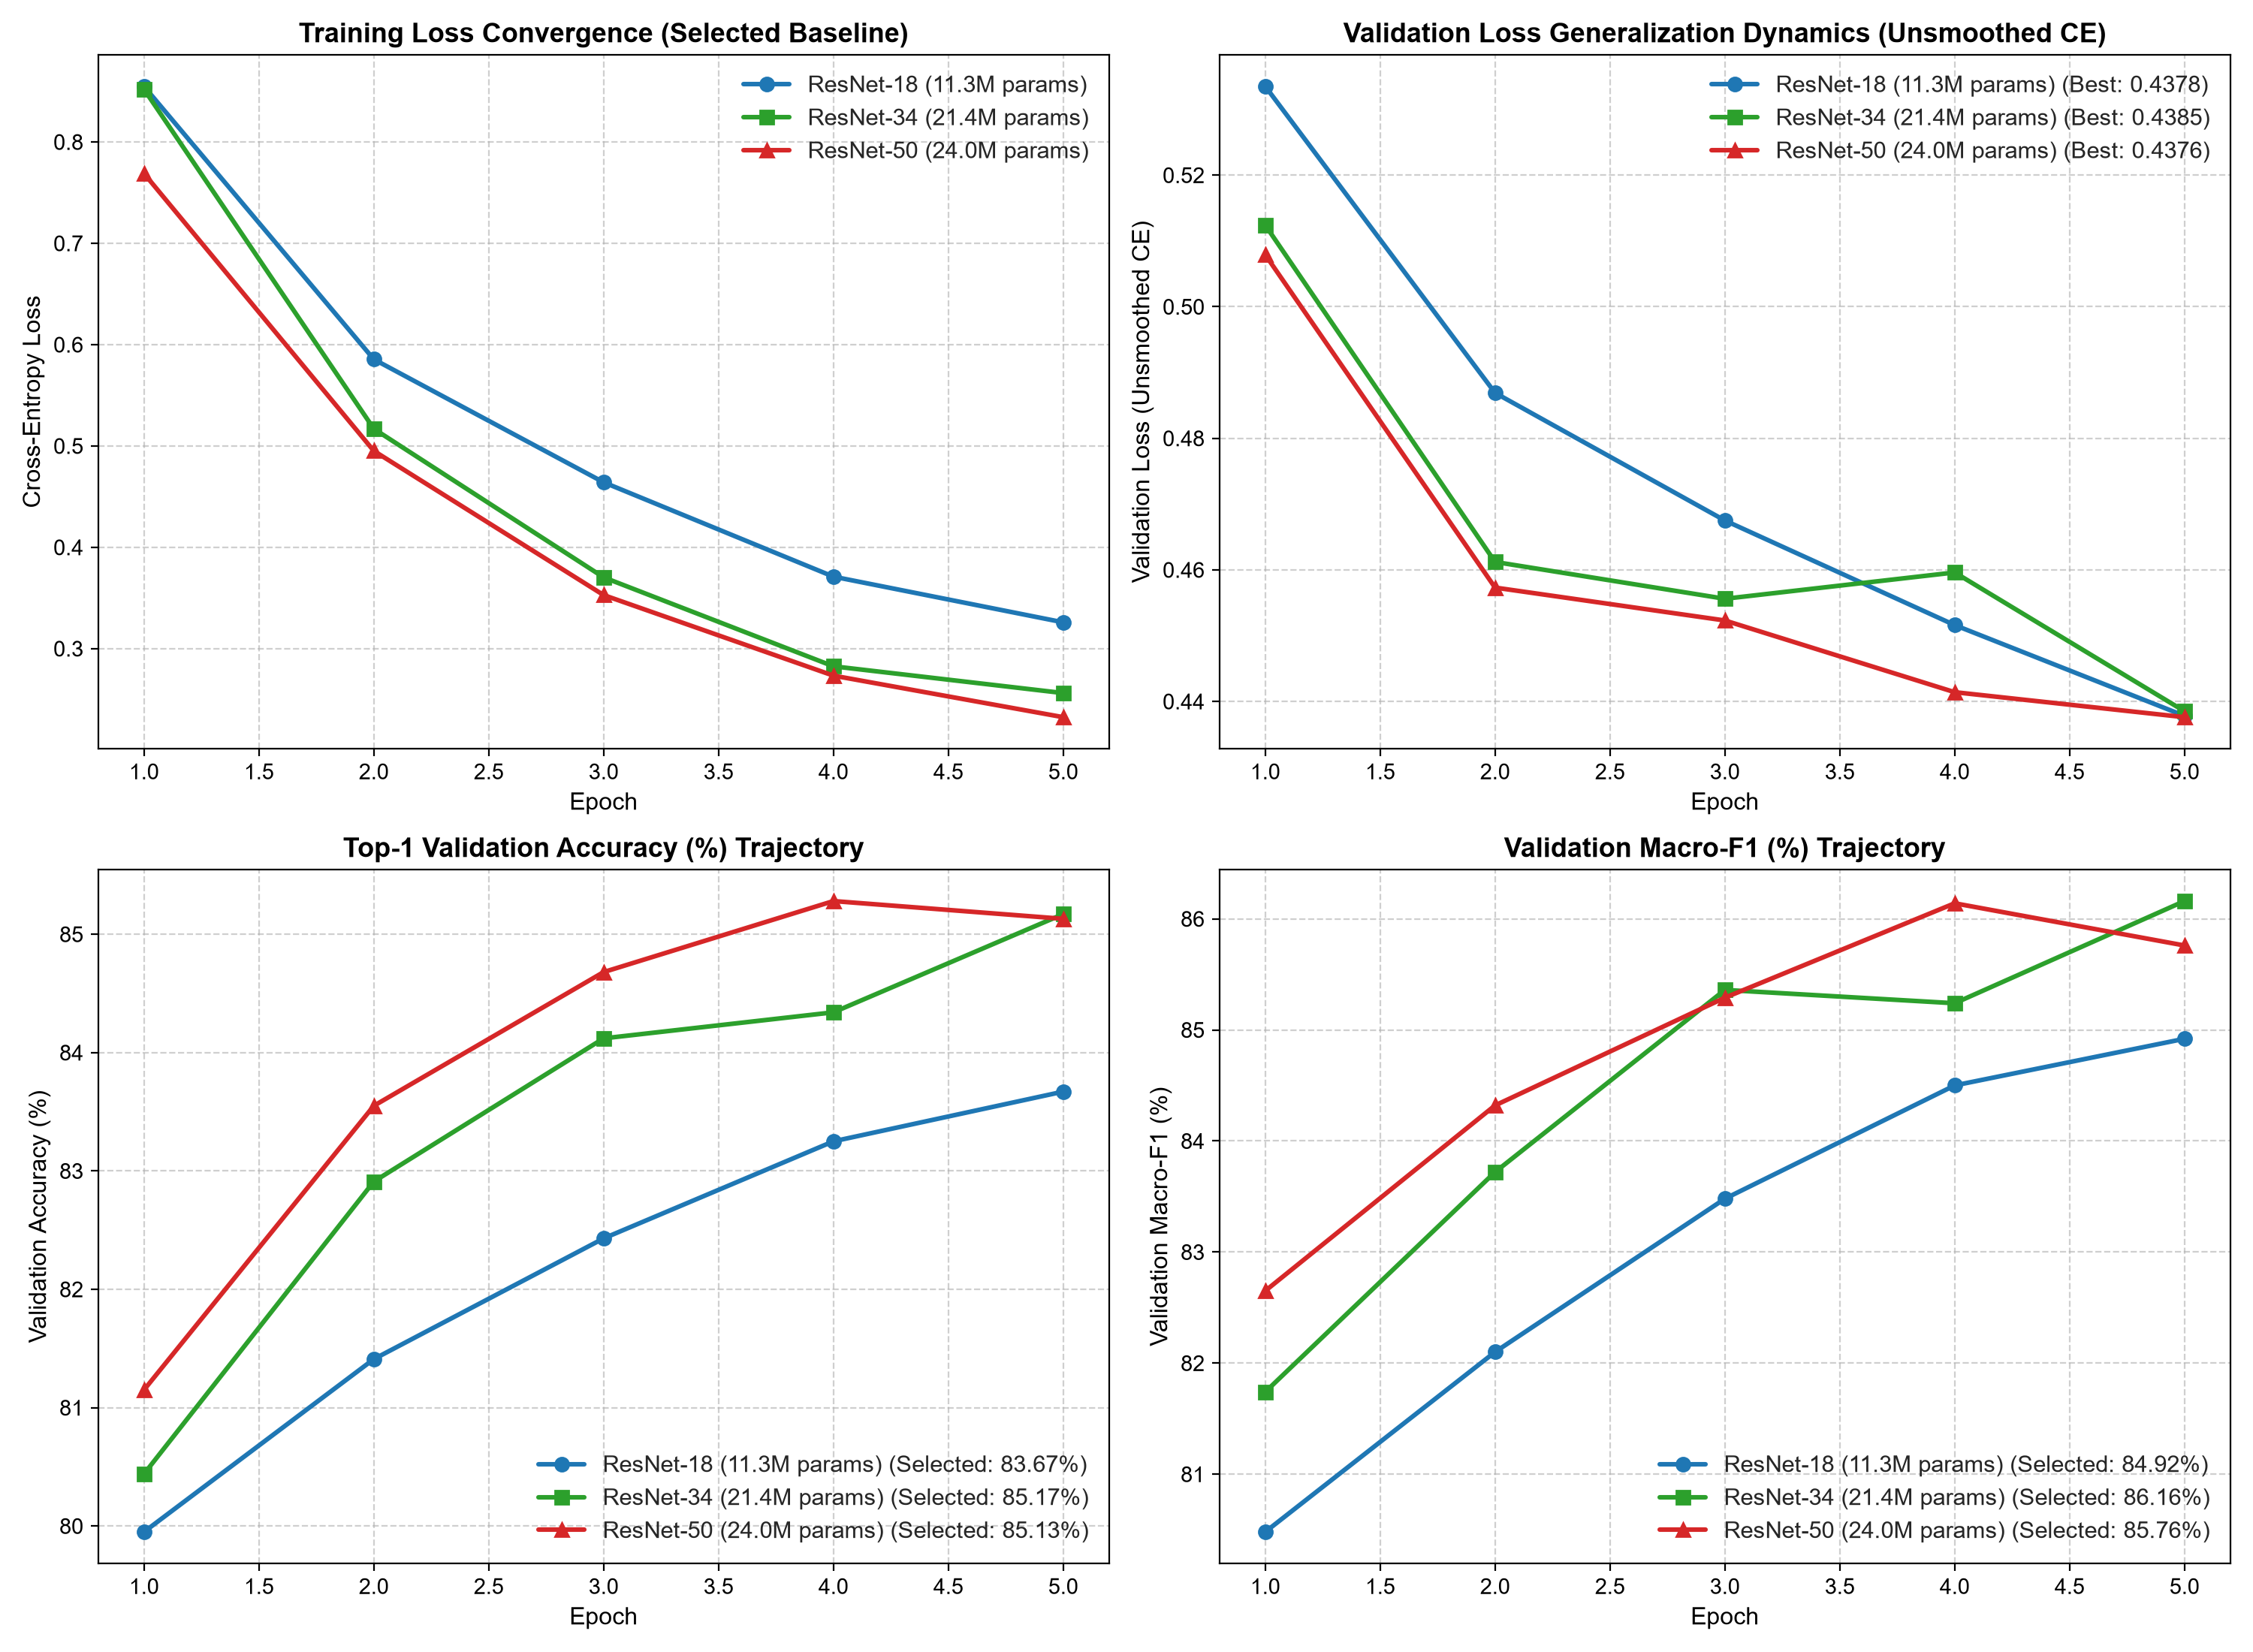
\includegraphics[width=0.76\linewidth]{figures/resnet_family_gradient_descent_comparison.png}
\caption{Gradient descent convergence dynamics across ResNet-18, ResNet-34, and ResNet-50 during 5-epoch Trial 08 screening runs on the internal development validation set. Panels display training loss convergence (top-left), unsmoothed validation loss (top-right), validation accuracy (bottom-left), and validation macro-F1 score (bottom-right). Legends indicate checkpoint-selected screening performance.}
\label{fig:family_convergence}
\end{figure}

The screening runs show that differential learning rates with AdamW ($\eta_{\text{bb}} = 5\times 10^{-5}, \eta_{\text{head}} = 5\times 10^{-4}$, Trial 08) outperform standard momentum SGD (Trial 04) by 1.2 to 2.0 percentage points across architectures (+1.5~pp for ResNet-18, +2.0~pp for ResNet-34, and +1.2~pp for ResNet-50). The unregularized label smoothing setting ($\alpha=0.0$) with weight decay $\lambda=1\times 10^{-2}$ yielded stable convergence across all three architectures and was selected as the baseline configuration for production benchmarks.

Separate per-pool hyperparameter tuning was then run for the CCSN-only and GCD-only pools using \texttt{--pool} in \texttt{tune\_resnet\_family.py}; the joint pool retained its approved configuration. The CCSN pool selected Trial 03 (aggressive AdamW, $\eta_{\text{bb}} = 1\times 10^{-4}$, $\eta_{\text{head}} = 1\times 10^{-3}$, label smoothing 0.1) for ResNet-18 and Trial 06 (weight decay $5\times 10^{-2}$) for ResNet-34 and ResNet-50. The GCD pool selected Trial 08 for all three architectures. Appendix~\ref{sec:appendix_tuning} lists the per-pool winning configurations and validation scores.

\section{Empirical Results and Comparative Production Benchmarks}
\label{sec:results}

\subsection{Evaluation Protocol}

Each production condition was trained under three seeds, $\{42,43,44\}$. Results are reported as mean $\pm$ across-seed sample standard deviation (ddof=1). No formal hypothesis test is applied; the dispersion reported here is seed-to-seed variation.

Two checkpoints were saved per run. The minimum-validation-loss checkpoint is the canonical selection criterion and is reported in the main text. The maximum-validation-macro-F1 checkpoint is used as a secondary diagnostic in Appendix~\ref{sec:appendix_master}. Earlier per-run bootstrap confidence intervals are superseded here by across-seed dispersion.

The CCSN-only arm was evaluated at 15 epochs and 90 epochs. The 90-epoch CCSN-only arm uses 2,160 optimizer steps, matching the joint model's per-source update budget (CCSN: 24 steps/epoch $\times$ 90 = 2,160; GCD-only and joint: 144 steps/epoch $\times$ 15 = 2,160). The 15-epoch CCSN-only arm (360 steps) remains as the unmatched-budget control.

An independent audit checked the benchmark code, tuned configs, per-run summaries, and artifact inventory with SHA-256 hashes. End-to-end reproduction runs matched the recorded metrics within across-seed variation. Runs are not bitwise deterministic.

\subsection{Primary Empirical Headline: Source-Balanced Joint Performance}

The headline benchmark result of this study is the joint CCSN+GCD model evaluated on the held-out test set, reported with source-balanced averaging across sensor modalities. Table~\ref{tab:primary_results} presents this primary comparison.

\begin{table}[!htbp]
\centering
\setlength{\tabcolsep}{8pt}
\begin{tabular}{lccccc}
\toprule
\textbf{Architecture} & \textbf{Params} & \textbf{CCSN} & \textbf{GCD} & \textbf{Source Avg} & \textbf{Pooled Test} \\
 & & ($n=468$) & ($n=2,862$) & \textbf{(Headline)} & ($n=3,330$) \\
\midrule
\textbf{ResNet-18} & 11.3M & $60.97 \pm 0.54$ & $87.22 \pm 1.77$ & $\mathbf{74.09 \pm 1.14}$ & $83.53 \pm 1.59$ \\
ResNet-34 & 21.4M & $59.90 \pm 2.48$ & $87.59 \pm 2.11$ & $73.74 \pm 2.20$ & $83.69 \pm 2.12$ \\
ResNet-50 & 24.0M & $61.54 \pm 2.94$ & $86.90 \pm 1.04$ & $74.22 \pm 1.97$ & $83.33 \pm 1.29$ \\
\bottomrule
\end{tabular}
\caption{Primary benchmark results on the held-out test set ($N=3,330$ images), using the joint model, minimum-validation-loss checkpoint, and three-seed mean $\pm$ across-seed SD. The headline metric is the unweighted arithmetic mean of the CCSN and GCD component accuracies, preventing the GCD sample volume ($n=2,862$) from dominating regional CCSN evaluation ($n=468$). The three architectures' source-balanced means fall within one standard deviation of one another.}
\label{tab:primary_results}
\end{table}

Table~\ref{tab:primary_results} gives three main comparisons:
\begin{enumerate}[noitemsep, topsep=2pt]
    \item Source-balanced accuracy is 74.1\%, 73.7\%, and 74.2\% for ResNet-18, ResNet-34, and ResNet-50. These differences are smaller than the across-seed standard deviation (1.1--2.2~pp). ResNet-18 is therefore adopted as the operating point on parameter and FLOP grounds: 53\% fewer parameters and 56\% fewer FLOPs than ResNet-50.
    \item On the pooled test set ($n=3,330$), the three architectures score $83.53 \pm 1.59$, $83.69 \pm 2.12$, and $83.33 \pm 1.29$. Because GCD contributes 85.95\% of the pooled test set, pooled accuracy mainly tracks whole-sky GCD performance. Source-balanced averaging gives the regional and whole-sky components equal weight.
    \item ResNet-50 has the highest CCSN component mean ($61.54 \pm 2.94$), while ResNet-18 and ResNet-34 have slightly higher GCD means ($87.22 \pm 1.77$ and $87.59 \pm 2.11$). The component-level spreads overlap across architectures.
\end{enumerate}

Figure~\ref{fig:cm_joint_pooled} details the class-level prediction distributions and errors of the adopted ResNet-18 joint model across this pooled test set.

\begin{figure}[!htbp]
\centering
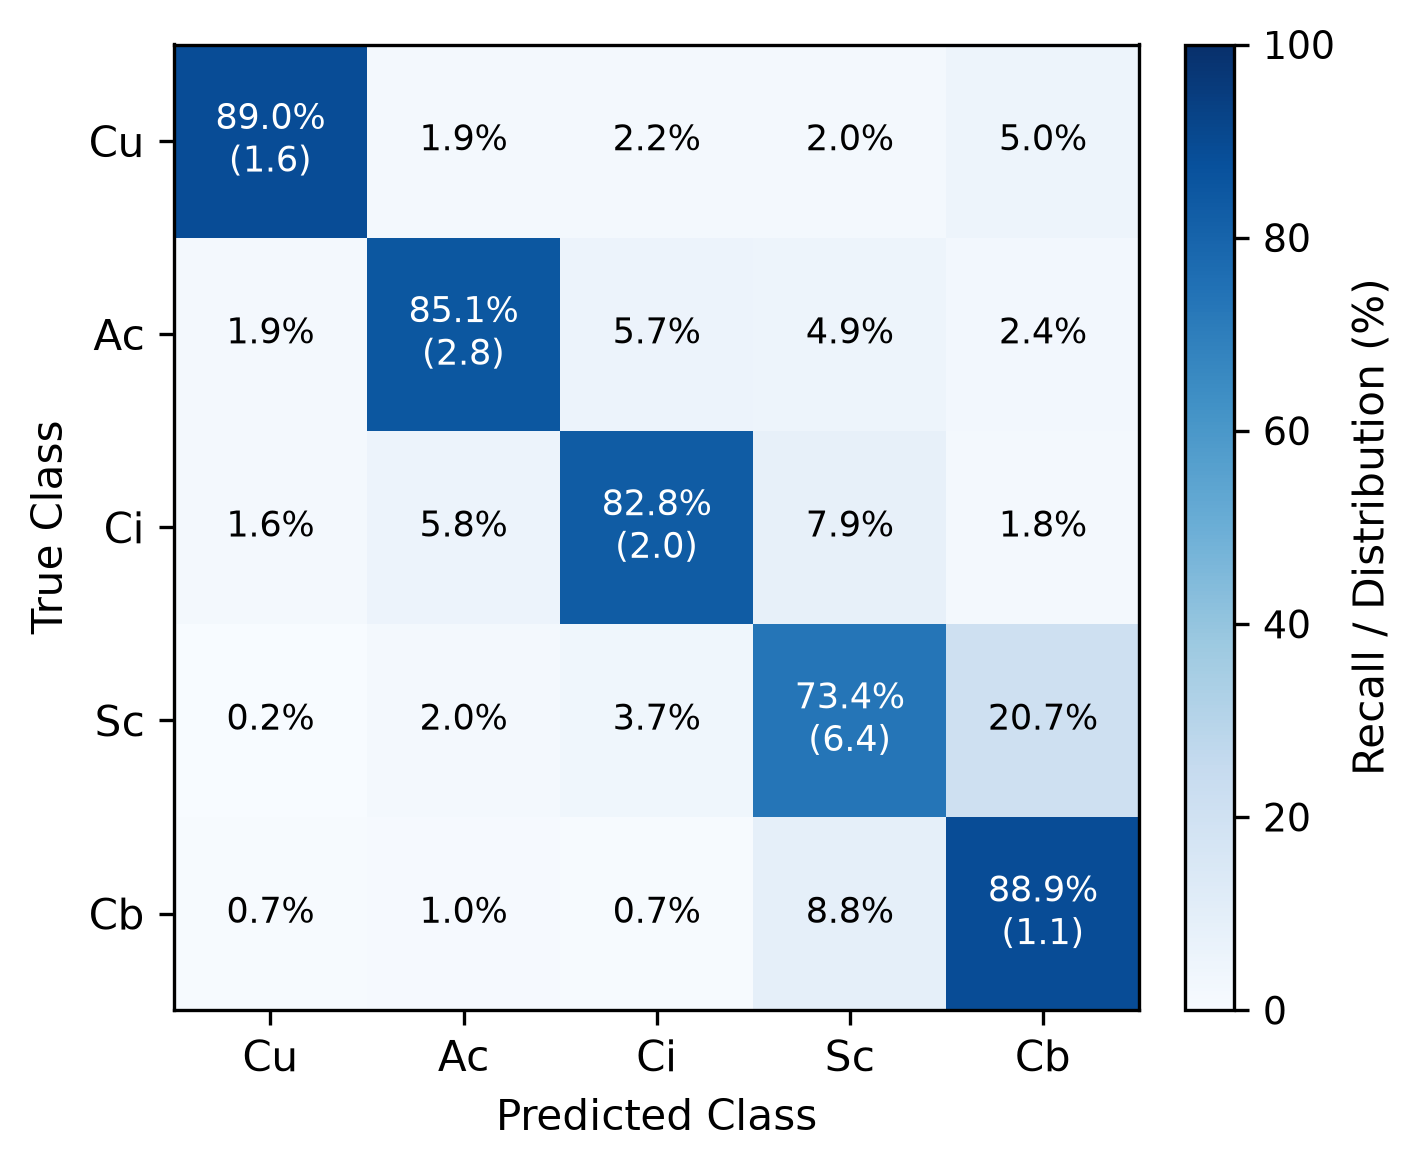
\includegraphics[width=0.55\textwidth]{figures/cm_joint_pooled_resnet18.png}
\caption{Row-normalized confusion matrix for the ResNet-18 joint model on the pooled five-class held-out test set ($N=3{,}330$), minimum-validation-loss checkpoint, three-seed mean; diagonal parentheses give the across-seed standard deviation.}
\label{fig:cm_joint_pooled}
\end{figure}

\subsection{Cross-Source Domain Discrepancy and Transfer Asymmetry}
\label{sec:cross_source_transfer}

Ground-based sky imaging archives collected under differing operational objectives exhibit domain shift across camera optics, sensor perspectives, and class frequencies. In the whole-sky GCD archive, Cumulonimbus represents 40.3\% of images (5,764 samples), whereas in regional CCSN views, Cumulonimbus accounts for 22.1\% (516 samples). Conversely, CCSN is dominated by Stratocumulus (31.2\%) and features twice the relative frequency of Altocumulus (20.8\% vs.\ 10.3\% in GCD). GCD contains over six times as many images as CCSN ($14,306$ vs.\ $2,337$), which motivates the inverse-volume batch sampling weights ($w_i = 0.5 / N_{\text{domain}(i)}$) defined in Section~\ref{sec:optimization}.

\begin{table}[!htbp]
\centering
\setlength{\tabcolsep}{8pt}
\begin{tabular}{llccc}
\toprule
\textbf{Direction} & \textbf{Metric} & \textbf{ResNet-18} & \textbf{ResNet-34} & \textbf{ResNet-50} \\
\midrule
CCSN$\to$GCD & Top-1 & $39.14 \pm 4.21$ & $40.67 \pm 0.99$ & $41.13 \pm 3.18$ \\
CCSN$\to$GCD & Macro-F1 & $44.03 \pm 4.13$ & $45.46 \pm 1.91$ & $43.13 \pm 0.52$ \\
GCD$\to$CCSN & Top-1 & $34.76 \pm 1.42$ & $36.61 \pm 1.17$ & $35.47 \pm 1.86$ \\
GCD$\to$CCSN & Macro-F1 & $33.60 \pm 1.80$ & $35.77 \pm 1.34$ & $34.63 \pm 1.82$ \\
\bottomrule
\end{tabular}
\caption{Cross-source transfer using single-source models, minimum-validation-loss checkpoint, and three-seed mean $\pm$ across-seed SD. The CCSN-only models use the CCSN-tuned configuration.}
\label{tab:transfer_summary}
\end{table}

Cross-source transfer is lossy in both directions: top-1 accuracy is about 35--41\% under transfer, compared with about 90\% for in-domain GCD evaluation. The regional-to-whole-sky direction is consistently 3--6~pp higher in top-1 accuracy and about 8--10~pp higher in macro-F1 across all three architectures. This directionality is smaller than the earlier single-configuration estimate because the CCSN-only models here use CCSN-tuned hyperparameters.

\begin{table}[!htbp]
\centering
\small
\setlength{\tabcolsep}{7pt}
\begin{tabular}{lccc}
\toprule
\textbf{Class} & \textbf{CCSN$\to$GCD Recall} & \textbf{GCD$\to$CCSN Recall} & \textbf{Paired Difference} \\
\midrule
Cumulus & $40.87 \pm 7.33$ & $68.52 \pm 3.20$ & $-27.65 \pm 9.99$ \\
Altocumulus & $65.88 \pm 4.43$ & $60.48 \pm 1.20$ & $5.40 \pm 3.27$ \\
Cirrus & $55.21 \pm 2.81$ & $53.73 \pm 2.96$ & $1.48 \pm 4.21$ \\
Stratocumulus & $57.01 \pm 18.88$ & $9.59 \pm 2.06$ & $47.42 \pm 19.53$ \\
Cumulonimbus & $15.26 \pm 1.46$ & $18.91 \pm 3.38$ & $-3.65 \pm 1.99$ \\
\bottomrule
\end{tabular}
\caption{ResNet-18 per-class recall under cross-source transfer, computed from the three per-seed summary files. Values are mean $\pm$ across-seed SD; paired differences subtract GCD$\to$CCSN from CCSN$\to$GCD.}
\label{tab:transfer_per_class}
\end{table}

While camera optics, field-of-view, and class distributions are known observational differences between the archives, attributing transfer differences to specific visual features remains an observational hypothesis rather than an isolated causal claim. Detailed per-condition metrics across the 36-run matrix are compiled in Appendix Tables~\ref{tab:production_master} and~\ref{tab:production_master_f1}.

\FloatBarrier
\section{Error Analysis: CCSN In-Domain Difficulty and the Role of Training Budget}
\label{sec:failure_modes}

\subsection{CCSN In-Domain Performance Across Recipes}

\begin{table}[!htbp]
\centering
\begin{tabular}{lccc}
\toprule
\textbf{Architecture} & \textbf{CCSN-15 Control} & \textbf{CCSN-90 Budget-Matched} & \textbf{Joint on CCSN} \\
\midrule
ResNet-18 & $58.90 \pm 0.96$ & $61.18 \pm 0.54$ & $60.97 \pm 0.54$ \\
ResNet-34 & $58.05 \pm 1.78$ & $57.48 \pm 1.62$ & $59.90 \pm 2.48$ \\
ResNet-50 & $59.12 \pm 1.37$ & $58.55 \pm 3.03$ & $61.54 \pm 2.94$ \\
\bottomrule
\end{tabular}
\caption{CCSN in-domain top-1 accuracy under three recipes, using the minimum-validation-loss checkpoint and three-seed mean $\pm$ across-seed SD.}
\label{tab:ccsn_recipes}
\end{table}

CCSN in-domain accuracy sits near 57--62\% under every recipe and architecture. Across-seed SD is usually 1--3~pp, comparable to the differences between recipes. The 468-image CCSN test component remains difficult regardless of training data mixture or optimizer-step budget.

\subsection{Budget-Matched Comparison}

\begin{table}[!htbp]
\centering
\small
\setlength{\tabcolsep}{5pt}
\begin{tabular}{llccc}
\toprule
\textbf{Arch.} & \textbf{Contrast} & \textbf{$\Delta$ Top-1} & \textbf{$\Delta$ Bal. Acc.} & \textbf{$\Delta$ Macro-F1} \\
\midrule
R18 & CCSN-90 $-$ CCSN-15 & $+2.28 \pm 1.25$ & $+2.08 \pm 0.67$ & $+2.23 \pm 1.46$ \\
R18 & Joint $-$ CCSN-90 & $-0.21 \pm 1.07$ & $+0.73 \pm 0.44$ & $+0.51 \pm 0.42$ \\
R18 & Joint $-$ CCSN-15 & $+2.07 \pm 0.81$ & $+2.81 \pm 0.71$ & $+2.74 \pm 1.03$ \\
R34 & CCSN-90 $-$ CCSN-15 & $-0.57 \pm 0.32$ & $-0.61 \pm 0.54$ & $-0.56 \pm 0.42$ \\
R34 & Joint $-$ CCSN-90 & $+2.42 \pm 0.99$ & $+3.00 \pm 1.74$ & $+3.09 \pm 1.65$ \\
R34 & Joint $-$ CCSN-15 & $+1.85 \pm 1.10$ & $+2.38 \pm 1.26$ & $+2.53 \pm 1.26$ \\
R50 & CCSN-90 $-$ CCSN-15 & $-0.57 \pm 3.51$ & $-2.89 \pm 1.81$ & $-2.47 \pm 1.77$ \\
R50 & Joint $-$ CCSN-90 & $+2.99 \pm 4.17$ & $+4.22 \pm 2.82$ & $+4.12 \pm 2.36$ \\
R50 & Joint $-$ CCSN-15 & $+2.42 \pm 1.61$ & $+1.33 \pm 1.27$ & $+1.64 \pm 0.64$ \\
\bottomrule
\end{tabular}
\caption{Paired-by-seed CCSN component differences, minimum-validation-loss checkpoint, $n=3$ seeds. Values are mean $\pm$ sample SD of the paired seed differences.}
\label{tab:budget_contrasts}
\end{table}

For ResNet-18, once the CCSN-only model receives the same 2,160-step budget as the joint model, the joint advantage disappears in top-1 accuracy ($-0.21 \pm 1.07$~pp). The apparent gain against the 15-epoch control ($+2.07 \pm 0.81$~pp) tracks the added optimization budget ($+2.28 \pm 1.25$~pp from budget alone).

For ResNet-34, joint training exceeds the budget-matched CCSN-only model by $+2.42 \pm 0.99$~pp top-1. The balanced-accuracy and macro-F1 differences ($+3.00 \pm 1.74$ and $+3.09 \pm 1.65$~pp) have standard deviations close to their means, so the effect remains suggestive. For ResNet-50, all contrasts have standard deviations larger than or comparable to their means. The small CCSN pool (1,495 training images) drives high seed variance in the deepest model. Overall, there is no architecture-independent joint-training benefit on the CCSN component after budget matching; the clearest case is ResNet-34, and it is modest.

\subsection{CCSN Class-Level Recall}

Figure~\ref{fig:cm_ccsn_shift} compares the class-level error distributions of the 15-epoch CCSN-only control and the joint model on the held-out CCSN test component, with per-class diagonal recall shifts summarized in Table~\ref{tab:ccsn_recall_shift}.

\begin{figure}[!htbp]
\centering
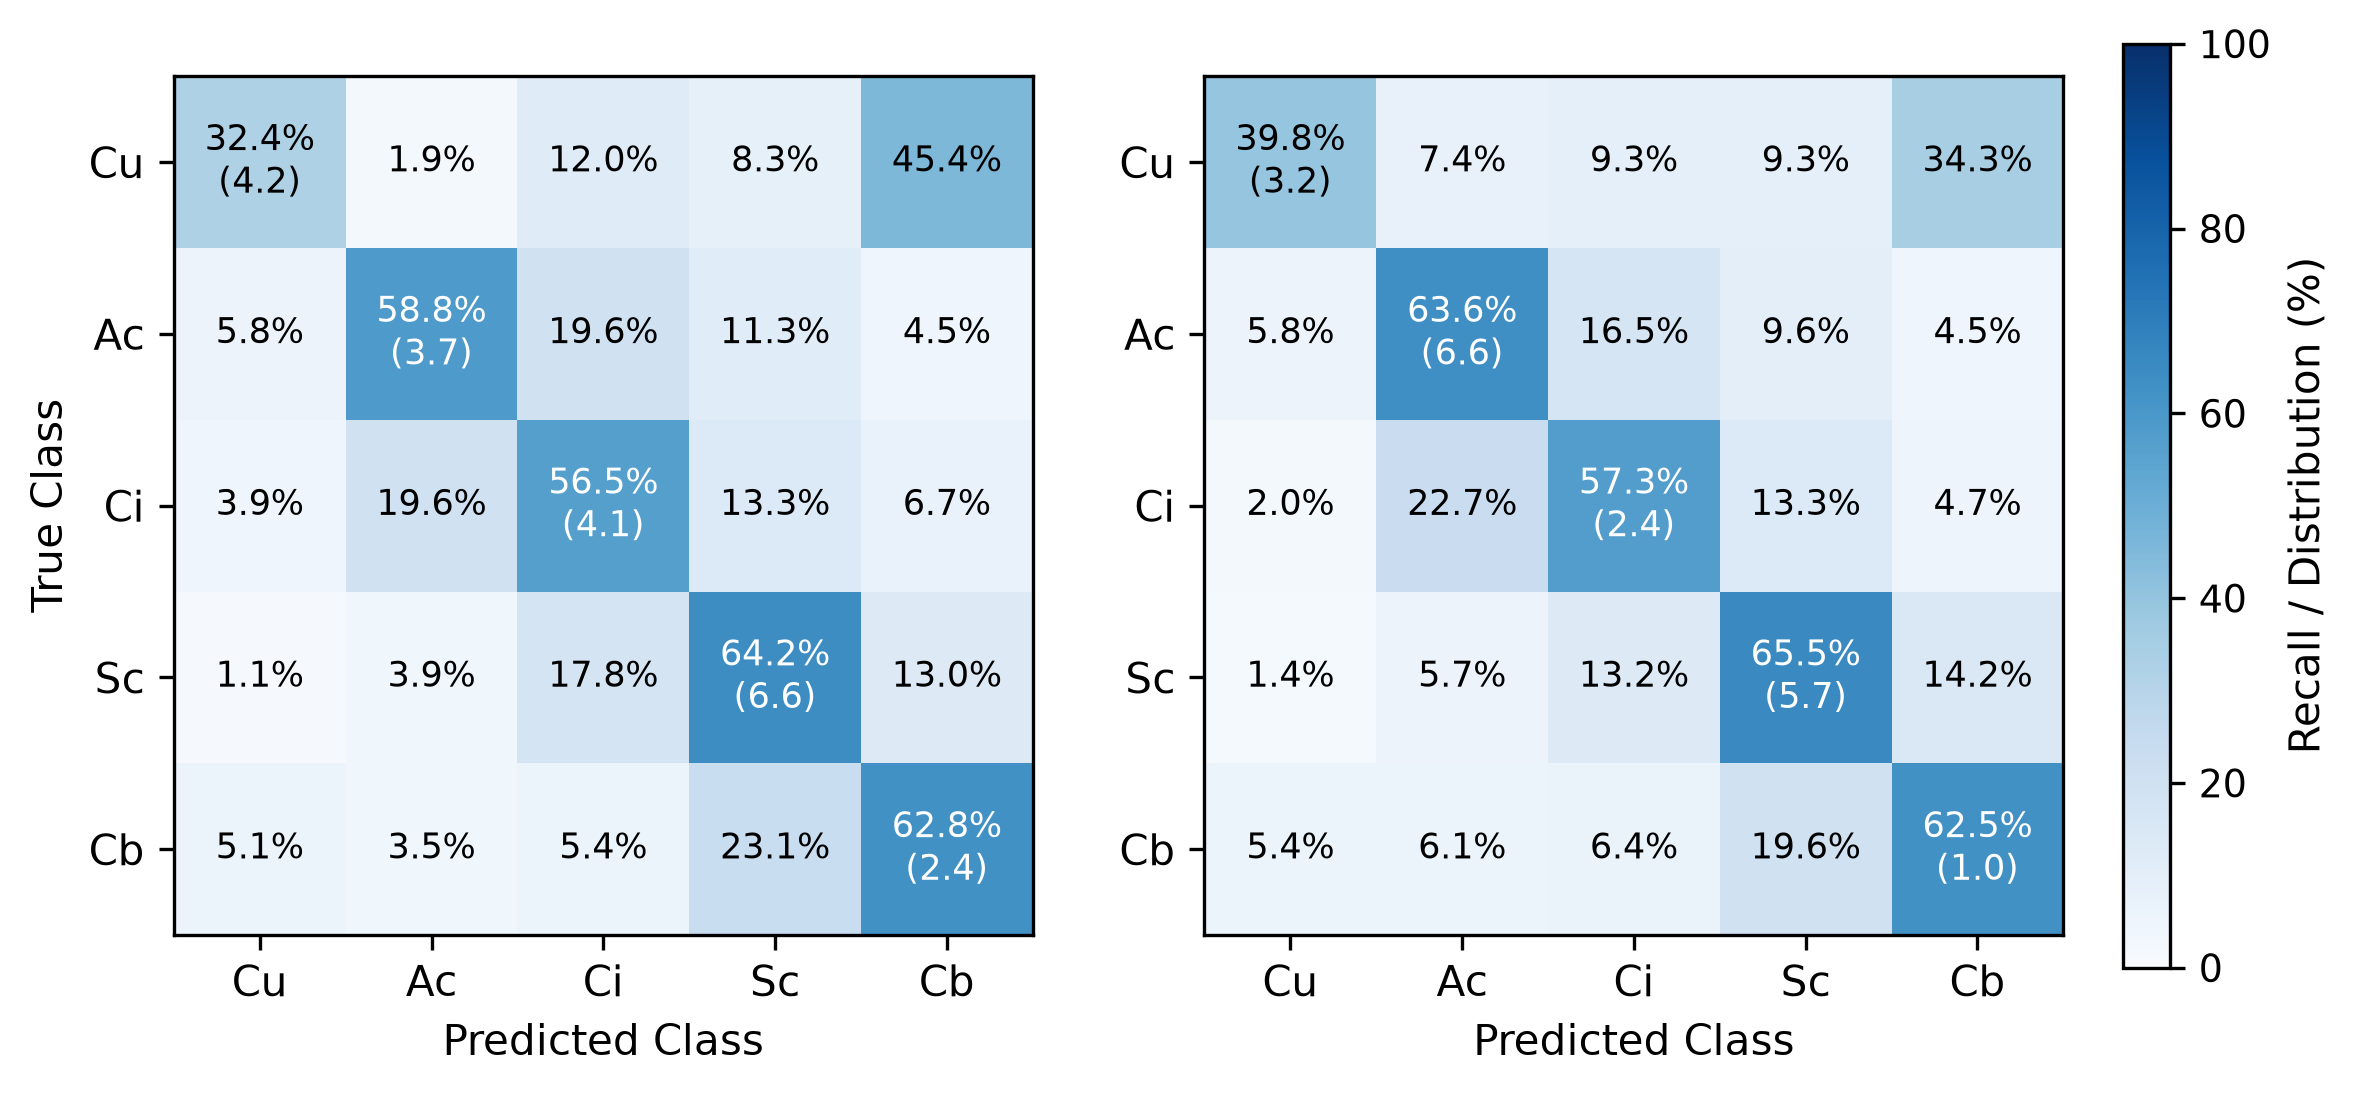
\includegraphics[width=0.92\textwidth]{figures/cm_ccsn_indomain_vs_joint_resnet18.png}
\caption{Row-normalized confusion matrices for ResNet-18 on the CCSN test component ($N=468$): 15-epoch CCSN-only control (left) versus the joint model (right), minimum-validation-loss checkpoint, three-seed mean.}
\label{fig:cm_ccsn_shift}
\end{figure}

\begin{table}[!htbp]
\centering
\small
\setlength{\tabcolsep}{7pt}
\begin{tabular}{lccc}
\toprule
\textbf{Class} & \textbf{CCSN-15 Recall} & \textbf{Joint Recall on CCSN} & \textbf{Paired Difference} \\
\midrule
Cumulus & $32.41 \pm 4.24$ & $39.82 \pm 3.21$ & $+7.41 \pm 6.99$ \\
Altocumulus & $58.76 \pm 3.72$ & $63.57 \pm 6.63$ & $+4.81 \pm 8.77$ \\
Cirrus & $56.47 \pm 4.08$ & $57.25 \pm 2.45$ & $+0.79 \pm 6.48$ \\
Stratocumulus & $64.15 \pm 6.58$ & $65.52 \pm 5.75$ & $+1.37 \pm 8.33$ \\
Cumulonimbus & $62.82 \pm 2.42$ & $62.50 \pm 0.96$ & $-0.32 \pm 1.47$ \\
\bottomrule
\end{tabular}
\caption{ResNet-18 CCSN per-class recall for the 15-epoch CCSN-only control and the joint model, using minimum-validation-loss checkpoints. Values are mean $\pm$ across-seed SD; paired differences subtract CCSN-15 recall from joint recall.}
\label{tab:ccsn_recall_shift}
\end{table}

\subsection{Persistent Failure Modes}

Key meteorological ambiguities remain:
\begin{enumerate}[noitemsep, topsep=2pt]
    \item Altocumulus ($C_2$) and Stratocumulus ($C_4$) still confuse one another because both can show layered roll textures during cloud transitions.
    \item Dense Stratocumulus decks cast dark grey diffuse lighting across ground sensors, visually resembling precipitation-bearing cloud bases ($C_5$) in single static frames without temporal, barometric, or radar data.
    \item Wide-angle sky imagery includes peripheral horizon clutter such as vegetation, masts, and local topography, none of which appears in the same way in regional sky views.
\end{enumerate}

\section{Conclusion and Future Work}
\label{sec:conclusion}

We studied deep residual networks for cross-source ground-based cloud classification. By identifying cross-split duplicate exposures in public releases and applying Stratified Group $K$-Fold, we set up benchmark splits that prevent duplicate leakage. We defined five shared cloud classes to combine regional digital camera and wide-angle whole-sky datasets, applied balanced batch sampling, and evaluated convergence across hyperparameter configurations. Joint training reaches about 74\% source-balanced accuracy for all three architectures, within seed variation; ResNet-18 is adopted as the lightweight operating point because it uses 53\% fewer parameters and 56\% fewer FLOPs than ResNet-50. After matching optimizer-step budget, joint training shows no consistent CCSN in-domain gain on ResNet-18 and a modest one on ResNet-34; CCSN in-domain accuracy is about 57--62\% across recipes. Cross-source transfer is lossy in both directions, with a small, consistent CCSN$\to$GCD $>$ GCD$\to$CCSN asymmetry.

\paragraph{Future Work}
With 11.3M parameters and 1.82~GFLOPs, ResNet-18 is well suited for resource-constrained meteorological stations and mobile sensing platforms. Future work should evaluate on-device latency, runtime memory consumption, and INT8 quantization on embedded field hardware.

\bibliographystyle{IEEEtran}
\begin{thebibliography}{99}
\footnotesize
\setlength{\itemsep}{-1pt}
\setlength{\parskip}{0pt}
\bibitem{stephens2005cloud}
G.~L. Stephens, ``Cloud feedbacks in the climate system: A critical review,'' \emph{Journal of Climate}, vol.~18, no.~2, pp. 237--273, 2005.
\bibitem{heinle2010automatic}
A.~Heinle, A.~Macke, and A.~Srivastav, ``Automatic cloud classification of whole sky images,'' \emph{Atmospheric Measurement Techniques}, vol.~3, no.~3, pp. 557--567, 2010.
\bibitem{wmo2017cloud}
World Meteorological Organization, \emph{Manual on the Observation of Clouds and Other Meteors (WMO-No. 407)}, International Cloud Atlas, Geneva, Switzerland, 2017.
\bibitem{zhang2018cloud}
J.~Zhang, P.~Liu, F.~Zhang, and Q.~Song, ``CloudNet: Ground-based cloud classification with deep convolutional neural networks,'' \emph{Geophysical Research Letters}, vol.~45, no.~16, pp. 8665--8672, 2018, doi: 10.1029/2018GL077787.
\bibitem{liu2022ground}
S.~Liu, M.~Li, Z.~Zhang, B.~Xiao, and X.~Cao, ``Ground-based remote sensing cloud classification via context graph attention network,'' \emph{IEEE Transactions on Geoscience and Remote Sensing}, vol.~60, pp. 1--11, Art no. 5602711, 2022, doi: 10.1109/TGRS.2021.3063255.
\bibitem{he2016deep}
K.~He, X.~Zhang, S.~Ren, and J.~Sun, ``Deep residual learning for image recognition,'' in \emph{Proceedings of the IEEE Conference on Computer Vision and Pattern Recognition (CVPR)}, pp. 770--778, 2016.
\end{thebibliography}

\clearpage
\appendix
\section*{Appendix A: Hyperparameter Exploration on Development Data}
\addcontentsline{toc}{section}{Appendix A: Hyperparameter Exploration on Development Data}
\label{sec:appendix_tuning}

Table~\ref{tab:tuning_results} documents empirical validation performance across the ten joint-pool hyperparameter exploration configurations evaluated on the internal development validation set ($N=2,663$ images). Sweeps explored differential learning rates, weight decay, label smoothing, and dropout regularization under AdamW and SGD with momentum. Trial 08 was selected as the joint production configuration.

\begin{table}[!htbp]
\centering
\small
\resizebox{\textwidth}{!}{%
\begin{tabular}{llcccccc}
\toprule
\textbf{Trial ID} & \textbf{Configuration Description} & \textbf{Optimizer} & \textbf{Backbone LR} & \textbf{Head LR} & \textbf{ResNet-18} & \textbf{ResNet-34} & \textbf{ResNet-50} \\
\midrule
Trial 01 & Baseline Differential LRs & AdamW & $5\times 10^{-5}$ & $5\times 10^{-4}$ & 84.3\% & 83.7\% & 84.9\% \\
Trial 02 & Conservative (Low LR) & AdamW & $2\times 10^{-5}$ & $2\times 10^{-4}$ & 83.3\% & 82.6\% & 83.1\% \\
Trial 03 & Aggressive (High LR) & AdamW & $1\times 10^{-4}$ & $1\times 10^{-3}$ & 84.4\% & 85.0\% & 85.9\% \\
Trial 04 & Standard Momentum & SGD & $1\times 10^{-3}$ & $1\times 10^{-2}$ & 82.2\% & 83.2\% & 83.9\% \\
Trial 05 & Conservative Momentum & SGD & $5\times 10^{-4}$ & $5\times 10^{-3}$ & 81.4\% & 82.0\% & 82.4\% \\
Trial 06 & High Weight Decay ($5\times 10^{-2}$) & AdamW & $5\times 10^{-5}$ & $5\times 10^{-4}$ & 84.6\% & 84.9\% & 83.8\% \\
Trial 07 & Low Weight Decay ($1\times 10^{-3}$) & AdamW & $5\times 10^{-5}$ & $5\times 10^{-4}$ & 83.9\% & 83.7\% & 84.8\% \\
Trial 08 & \textbf{Standard LRs (LS 0.0)} & \textbf{AdamW} & $\mathbf{5\times 10^{-5}}$ & $\mathbf{5\times 10^{-4}}$ & \textbf{83.7\%} & \textbf{85.2\%} & \textbf{85.1\%} \\
Trial 09 & Heavy Dropout ($0.4 / 0.5$) & AdamW & $5\times 10^{-5}$ & $5\times 10^{-4}$ & 85.4\% & 84.8\% & 85.7\% \\
Trial 10 & Fine Differential ($4\times 10^{-5} / 4\times 10^{-4}$) & AdamW & $4\times 10^{-5}$ & $4\times 10^{-4}$ & 84.5\% & 84.1\% & 85.1\% \\
\bottomrule
\end{tabular}%
}
\caption{Empirical validation accuracy across 10 hyperparameter exploration configurations on the internal development validation set (2,663 images). Displayed values reflect 5-epoch screening runs scored on unsmoothed validation cross-entropy loss.}
\label{tab:tuning_results}
\end{table}

\begin{table}[!htbp]
\centering
\small
\setlength{\tabcolsep}{5pt}
\resizebox{\textwidth}{!}{%
\begin{tabular}{lllccl}
\toprule
\textbf{Architecture} & \textbf{Pool} & \textbf{Winning Trial} & \textbf{Best Val Loss} & \textbf{Best Val Acc.} & \textbf{Best Val Macro-F1} \\
\midrule
ResNet-18 & CCSN & Trial 03, Aggressive AdamW & 1.0460 & 60.43 & 56.98 \\
ResNet-18 & GCD & Trial 08, AdamW + No Label Smoothing & 0.2609 & 88.60 & 90.77 \\
ResNet-34 & CCSN & Trial 06, AdamW + High Weight Decay & 1.0231 & 60.96 & 58.39 \\
ResNet-34 & GCD & Trial 08, AdamW + No Label Smoothing & 0.2678 & 89.25 & 91.03 \\
ResNet-50 & CCSN & Trial 06, AdamW + High Weight Decay & 1.0029 & 60.96 & 57.16 \\
ResNet-50 & GCD & Trial 08, AdamW + No Label Smoothing & 0.2459 & 89.86 & 91.66 \\
\bottomrule
\end{tabular}% 
}
\caption{Per-pool winning trials used by the single-source production configs. Validation metrics come from the corresponding \texttt{artifacts/tuning/tuning\_results\_*} JSON files.}
\label{tab:per_pool_tuning_results}
\end{table}

\clearpage
\section*{Appendix B: Production Benchmark Reference}
\addcontentsline{toc}{section}{Appendix B: Production Benchmark Reference}
\label{sec:appendix_master}

Table~\ref{tab:production_master} reports the canonical 27-condition benchmark across all architectures, single-source in-domain baselines, cross-source transfer evaluations, the 90-epoch CCSN budget arm, and joint models on the held-out test set ($N=3,330$ images). Values are three-seed means with across-seed SD for the minimum-validation-loss checkpoint.

\begin{table}[!htbp]
\centering
\scriptsize
\setlength{\tabcolsep}{4pt}
\renewcommand{\arraystretch}{0.9}
\resizebox{\textwidth}{!}{%
\begin{tabular}{llcccc}
\toprule
\textbf{Model Architecture} & \textbf{Experimental Condition} & \textbf{Evaluation Set} & \textbf{Top-1 Acc (\%)} & \textbf{Balanced Acc (\%)} & \textbf{Macro-F1 (\%)} \\
\midrule
\multirow{9}{*}{\textbf{ResNet-18} (11.3M)} 
& 1. CCSN-15 & CCSN Test Component & $58.90 \pm 0.96$ & $54.93 \pm 0.47$ & $55.28 \pm 1.02$ \\
& 2. CCSN-15 $\to$ GCD & GCD Test Component & $39.14 \pm 4.21$ & $46.85 \pm 3.55$ & $44.03 \pm 4.13$ \\
& 3. CCSN-90 & CCSN Test Component & $61.18 \pm 0.54$ & $57.00 \pm 0.25$ & $57.51 \pm 0.43$ \\
& 4. GCD-15 & GCD Test Component & $89.88 \pm 0.20$ & $92.10 \pm 0.29$ & $91.74 \pm 0.13$ \\
& 5. GCD-15 $\to$ CCSN & CCSN Test Component & $34.76 \pm 1.42$ & $42.24 \pm 1.36$ & $33.60 \pm 1.80$ \\
& 6. Joint & CCSN Test Component & $60.97 \pm 0.54$ & $57.73 \pm 0.31$ & $58.02 \pm 0.03$ \\
& 7. Joint & GCD Test Component & $87.22 \pm 1.77$ & $88.35 \pm 1.87$ & $88.85 \pm 1.81$ \\
& 8. Joint & Pooled Test Set & $83.53 \pm 1.59$ & $83.84 \pm 1.48$ & $84.22 \pm 1.61$ \\
& 9. Joint & \textbf{Source-Balanced Avg} & $\mathbf{74.09 \pm 1.14}$ & $\mathbf{73.04 \pm 0.80}$ & $\mathbf{73.44 \pm 0.89}$ \\
\midrule
\multirow{9}{*}{\textbf{ResNet-34} (21.4M)} 
& 1. CCSN-15 & CCSN Test Component & $58.05 \pm 1.78$ & $55.74 \pm 0.65$ & $55.35 \pm 0.88$ \\
& 2. CCSN-15 $\to$ GCD & GCD Test Component & $40.67 \pm 0.99$ & $49.74 \pm 2.52$ & $45.46 \pm 1.91$ \\
& 3. CCSN-90 & CCSN Test Component & $57.48 \pm 1.62$ & $55.12 \pm 0.70$ & $54.79 \pm 0.50$ \\
& 4. GCD-15 & GCD Test Component & $89.33 \pm 0.47$ & $91.08 \pm 0.23$ & $90.97 \pm 0.29$ \\
& 5. GCD-15 $\to$ CCSN & CCSN Test Component & $36.61 \pm 1.17$ & $44.47 \pm 1.29$ & $35.77 \pm 1.34$ \\
& 6. Joint & CCSN Test Component & $59.90 \pm 2.48$ & $58.12 \pm 1.29$ & $57.88 \pm 2.14$ \\
& 7. Joint & GCD Test Component & $87.59 \pm 2.11$ & $88.70 \pm 3.12$ & $88.89 \pm 2.94$ \\
& 8. Joint & Pooled Test Set & $83.69 \pm 2.12$ & $84.23 \pm 2.56$ & $84.20 \pm 2.78$ \\
& 9. Joint & \textbf{Source-Balanced Avg} & $73.74 \pm 2.20$ & $73.41 \pm 2.15$ & $73.39 \pm 2.48$ \\
\midrule
\multirow{9}{*}{\textbf{ResNet-50} (24.0M)} 
& 1. CCSN-15 & CCSN Test Component & $59.12 \pm 1.37$ & $57.70 \pm 1.77$ & $57.24 \pm 1.43$ \\
& 2. CCSN-15 $\to$ GCD & GCD Test Component & $41.13 \pm 3.18$ & $48.68 \pm 0.90$ & $43.13 \pm 0.52$ \\
& 3. CCSN-90 & CCSN Test Component & $58.55 \pm 3.03$ & $54.81 \pm 2.70$ & $54.77 \pm 2.48$ \\
& 4. GCD-15 & GCD Test Component & $89.49 \pm 0.40$ & $91.45 \pm 0.38$ & $91.37 \pm 0.13$ \\
& 5. GCD-15 $\to$ CCSN & CCSN Test Component & $35.47 \pm 1.86$ & $43.76 \pm 3.15$ & $34.63 \pm 1.82$ \\
& 6. Joint & CCSN Test Component & $61.54 \pm 2.94$ & $59.03 \pm 1.01$ & $58.89 \pm 1.72$ \\
& 7. Joint & GCD Test Component & $86.90 \pm 1.04$ & $88.15 \pm 1.37$ & $88.72 \pm 1.11$ \\
& 8. Joint & Pooled Test Set & $83.33 \pm 1.29$ & $83.80 \pm 1.31$ & $84.26 \pm 1.31$ \\
& 9. Joint & \textbf{Source-Balanced Avg} & $\mathbf{74.22 \pm 1.97}$ & $73.59 \pm 1.17$ & $73.80 \pm 1.41$ \\
\bottomrule
\end{tabular}%
}
\caption{Twenty-seven conditions (three architectures $\times$ nine evaluation conditions), three seeds each, minimum-validation-loss checkpoint, mean $\pm$ across-seed SD.}
\label{tab:production_master}
\end{table}

Table~\ref{tab:production_master_f1} repeats the benchmark for the maximum-validation-macro-F1 checkpoint. Under max-F1 selection, the joint-minus-budget-matched differences are larger for some metrics, for example ResNet-18 balanced accuracy $+3.84 \pm 0.42$~pp and macro-F1 $+3.61 \pm 0.31$~pp. This checkpoint sensitivity is why the minimum-validation-loss result remains canonical.

\begin{table}[!htbp]
\centering
\scriptsize
\setlength{\tabcolsep}{4pt}
\renewcommand{\arraystretch}{0.9}
\resizebox{\textwidth}{!}{%
\begin{tabular}{llcccc}
\toprule
\textbf{Model Architecture} & \textbf{Experimental Condition} & \textbf{Evaluation Set} & \textbf{Top-1 Acc (\%)} & \textbf{Balanced Acc (\%)} & \textbf{Macro-F1 (\%)} \\
\midrule
\multirow{9}{*}{\textbf{ResNet-18} (11.3M)} 
& 1. CCSN-15 & CCSN Test Component & $59.62 \pm 0.37$ & $56.24 \pm 0.88$ & $56.50 \pm 0.57$ \\
& 2. CCSN-15 $\to$ GCD & GCD Test Component & $38.82 \pm 2.64$ & $46.44 \pm 2.10$ & $44.10 \pm 2.19$ \\
& 3. CCSN-90 & CCSN Test Component & $60.82 \pm 0.86$ & $55.84 \pm 1.65$ & $56.21 \pm 1.47$ \\
& 4. GCD-15 & GCD Test Component & $89.68 \pm 0.41$ & $91.68 \pm 0.66$ & $91.53 \pm 0.31$ \\
& 5. GCD-15 $\to$ CCSN & CCSN Test Component & $34.90 \pm 1.55$ & $42.37 \pm 1.51$ & $33.72 \pm 1.92$ \\
& 6. Joint & CCSN Test Component & $62.32 \pm 1.42$ & $59.68 \pm 1.73$ & $59.81 \pm 1.36$ \\
& 7. Joint & GCD Test Component & $88.76 \pm 0.30$ & $90.29 \pm 0.25$ & $90.47 \pm 0.23$ \\
& 8. Joint & Pooled Test Set & $85.05 \pm 0.11$ & $85.66 \pm 0.16$ & $85.78 \pm 0.12$ \\
& 9. Joint & \textbf{Source-Balanced Avg} & $\mathbf{75.54 \pm 0.58}$ & $\mathbf{74.99 \pm 0.75}$ & $\mathbf{75.14 \pm 0.59}$ \\
\midrule
\multirow{9}{*}{\textbf{ResNet-34} (21.4M)}
& 1. CCSN-15 & CCSN Test Component & $57.91 \pm 1.07$ & $55.86 \pm 0.72$ & $55.53 \pm 1.10$ \\
& 2. CCSN-15 $\to$ GCD & GCD Test Component & $37.80 \pm 4.06$ & $46.79 \pm 4.42$ & $42.06 \pm 4.37$ \\
& 3. CCSN-90 & CCSN Test Component & $58.26 \pm 1.71$ & $53.56 \pm 0.90$ & $53.46 \pm 0.62$ \\
& 4. GCD-15 & GCD Test Component & $89.19 \pm 0.53$ & $91.16 \pm 0.75$ & $90.95 \pm 0.69$ \\
& 5. GCD-15 $\to$ CCSN & CCSN Test Component & $36.25 \pm 1.01$ & $44.92 \pm 1.70$ & $35.19 \pm 0.92$ \\
& 6. Joint & CCSN Test Component & $60.97 \pm 0.65$ & $58.31 \pm 0.91$ & $58.59 \pm 0.67$ \\
& 7. Joint & GCD Test Component & $88.89 \pm 0.24$ & $90.49 \pm 0.34$ & $90.67 \pm 0.26$ \\
& 8. Joint & Pooled Test Set & $84.96 \pm 0.13$ & $85.61 \pm 0.22$ & $85.84 \pm 0.15$ \\
& 9. Joint & \textbf{Source-Balanced Avg} & $74.93 \pm 0.22$ & $74.40 \pm 0.43$ & $74.63 \pm 0.34$ \\
\midrule
\multirow{9}{*}{\textbf{ResNet-50} (24.0M)}
& 1. CCSN-15 & CCSN Test Component & $61.04 \pm 1.01$ & $59.30 \pm 1.15$ & $59.10 \pm 1.31$ \\
& 2. CCSN-15 $\to$ GCD & GCD Test Component & $41.00 \pm 2.15$ & $46.61 \pm 2.67$ & $40.64 \pm 2.72$ \\
& 3. CCSN-90 & CCSN Test Component & $60.47 \pm 2.89$ & $57.88 \pm 1.30$ & $57.73 \pm 2.06$ \\
& 4. GCD-15 & GCD Test Component & $89.73 \pm 0.68$ & $91.71 \pm 0.67$ & $91.61 \pm 0.48$ \\
& 5. GCD-15 $\to$ CCSN & CCSN Test Component & $35.54 \pm 1.94$ & $43.50 \pm 2.87$ & $34.47 \pm 1.66$ \\
& 6. Joint & CCSN Test Component & $61.90 \pm 1.63$ & $57.43 \pm 1.03$ & $57.59 \pm 1.06$ \\
& 7. Joint & GCD Test Component & $89.66 \pm 0.28$ & $91.35 \pm 0.26$ & $91.42 \pm 0.32$ \\
& 8. Joint & Pooled Test Set & $85.76 \pm 0.47$ & $86.17 \pm 0.36$ & $86.52 \pm 0.47$ \\
& 9. Joint & \textbf{Source-Balanced Avg} & $\mathbf{75.78 \pm 0.96}$ & $74.39 \pm 0.58$ & $74.51 \pm 0.58$ \\
\bottomrule
\end{tabular}%
}
\caption{Same 27-condition layout as Table~\ref{tab:production_master}, using the maximum-validation-macro-F1 checkpoint. These values are a secondary diagnostic, not the primary protocol.}
\label{tab:production_master_f1}
\end{table}

\end{document}
